\documentclass[1p]{elsarticle_modified}
%\bibliographystyle{elsarticle-num}

%\usepackage[colorlinks]{hyperref}
%\usepackage{abbrmath_seonhwa} %\Abb, \Ascr, \Acal ,\Abf, \Afrak
\usepackage{amsfonts}
\usepackage{amssymb}
\usepackage{amsmath}
\usepackage{amsthm}
\usepackage{scalefnt}
\usepackage{amsbsy}
\usepackage{kotex}
\usepackage{caption}
\usepackage{subfig}
\usepackage{color}
\usepackage{graphicx}
\usepackage{xcolor} %% white, black, red, green, blue, cyan, magenta, yellow
\usepackage{float}
\usepackage{setspace}
\usepackage{hyperref}

\usepackage{tikz}
\usetikzlibrary{arrows}

\usepackage{multirow}
\usepackage{array} % fixed length table
\usepackage{hhline}

%%%%%%%%%%%%%%%%%%%%%
\makeatletter
\renewcommand*\env@matrix[1][\arraystretch]{%
	\edef\arraystretch{#1}%
	\hskip -\arraycolsep
	\let\@ifnextchar\new@ifnextchar
	\array{*\c@MaxMatrixCols c}}
\makeatother %https://tex.stackexchange.com/questions/14071/how-can-i-increase-the-line-spacing-in-a-matrix
%%%%%%%%%%%%%%%

\usepackage[normalem]{ulem}

\newcommand{\msout}[1]{\ifmmode\text{\sout{\ensuremath{#1}}}\else\sout{#1}\fi}
%SOURCE: \msout is \stkout macro in https://tex.stackexchange.com/questions/20609/strikeout-in-math-mode

\newcommand{\cancel}[1]{
	\ifmmode
	{\color{red}\msout{#1}}
	\else
	{\color{red}\sout{#1}}
	\fi
}

\newcommand{\add}[1]{
	{\color{blue}\uwave{#1}}
}

\newcommand{\replace}[2]{
	\ifmmode
	{\color{red}\msout{#1}}{\color{blue}\uwave{#2}}
	\else
	{\color{red}\sout{#1}}{\color{blue}\uwave{#2}}
	\fi
}

\newcommand{\Sol}{\mathcal{S}} %segment
\newcommand{\D}{D} %diagram
\newcommand{\A}{\mathcal{A}} %arc


%%%%%%%%%%%%%%%%%%%%%%%%%%%%%5 test

\def\sl{\operatorname{\textup{SL}}(2,\Cbb)}
\def\psl{\operatorname{\textup{PSL}}(2,\Cbb)}
\def\quan{\mkern 1mu \triangleright \mkern 1mu}

\theoremstyle{definition}
\newtheorem{thm}{Theorem}[section]
\newtheorem{prop}[thm]{Proposition}
\newtheorem{lem}[thm]{Lemma}
\newtheorem{ques}[thm]{Question}
\newtheorem{cor}[thm]{Corollary}
\newtheorem{defn}[thm]{Definition}
\newtheorem{exam}[thm]{Example}
\newtheorem{rmk}[thm]{Remark}
\newtheorem{alg}[thm]{Algorithm}

\newcommand{\I}{\sqrt{-1}}
\begin{document}

%\begin{frontmatter}
%
%\title{Boundary parabolic representations of knots up to 8 crossings}
%
%%% Group authors per affiliation:
%\author{Yunhi Cho} 
%\address{Department of Mathematics, University of Seoul, Seoul, Korea}
%\ead{yhcho@uos.ac.kr}
%
%
%\author{Seonhwa Kim} %\fnref{s_kim}}
%\address{Center for Geometry and Physics, Institute for Basic Science, Pohang, 37673, Korea}
%\ead{ryeona17@ibs.re.kr}
%
%\author{Hyuk Kim}
%\address{Department of Mathematical Sciences, Seoul National University, Seoul 08826, Korea}
%\ead{hyukkim@snu.ac.kr}
%
%\author{Seokbeom Yoon}
%\address{Department of Mathematical Sciences, Seoul National University, Seoul, 08826,  Korea}
%\ead{sbyoon15@snu.ac.kr}
%
%\begin{abstract}
%We find all boundary parabolic representation of knots up to 8 crossings.
%
%\end{abstract}
%\begin{keyword}
%    \MSC[2010] 57M25 
%\end{keyword}
%
%\end{frontmatter}

%\linenumbers
%\tableofcontents
%
\newcommand\colored[1]{\textcolor{white}{\rule[-0.35ex]{0.8em}{1.4ex}}\kern-0.8em\color{red} #1}%
%\newcommand\colored[1]{\textcolor{white}{ #1}\kern-2.17ex	\textcolor{white}{ #1}\kern-1.81ex	\textcolor{white}{ #1}\kern-2.15ex\color{red}#1	}

{\Large $\underline{12a_{0899}~(K12a_{0899})}$}

\setlength{\tabcolsep}{10pt}
\renewcommand{\arraystretch}{1.6}
\vspace{1cm}\begin{tabular}{m{100pt}>{\centering\arraybackslash}m{274pt}}
\multirow{5}{120pt}{
	\centering
	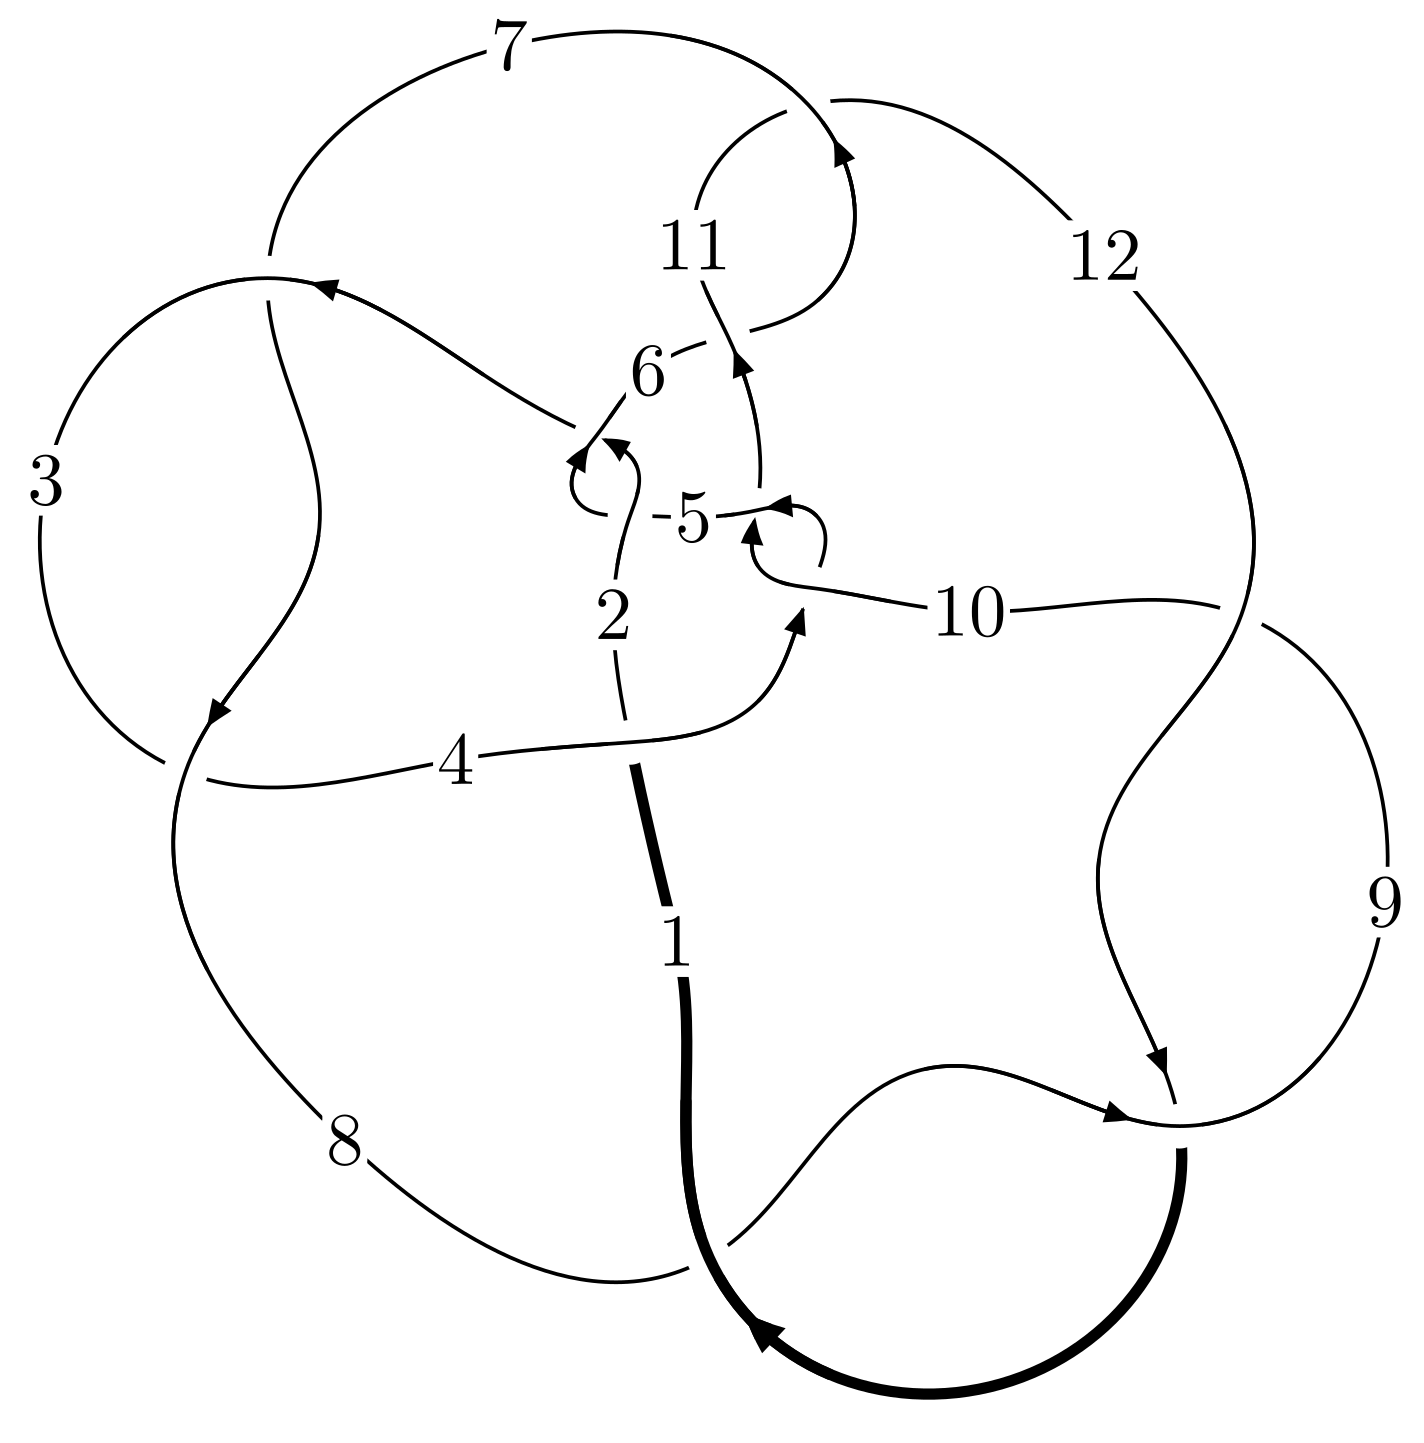
\includegraphics[width=112pt]{../../../GIT/diagram.site/Diagrams/png/1700_12a_0899.png}\\
\ \ \ A knot diagram\footnotemark}&
\allowdisplaybreaks
\textbf{Linearized knot diagam} \\
\cline{2-2}
 &
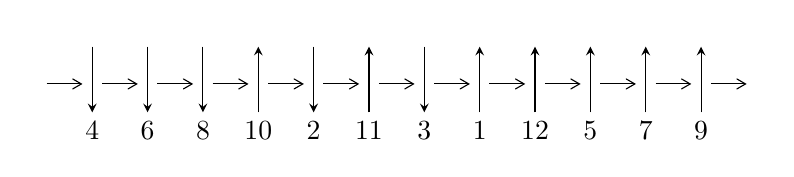
\begin{tikzpicture}[x=20pt, y=17pt]
	% nodes
	\node (C0) at (0, 0) {};
	\node (C1) at (1, 0) {};
	\node (C1U) at (1, +1) {};
	\node (C1D) at (1, -1) {4};

	\node (C2) at (2, 0) {};
	\node (C2U) at (2, +1) {};
	\node (C2D) at (2, -1) {6};

	\node (C3) at (3, 0) {};
	\node (C3U) at (3, +1) {};
	\node (C3D) at (3, -1) {8};

	\node (C4) at (4, 0) {};
	\node (C4U) at (4, +1) {};
	\node (C4D) at (4, -1) {10};

	\node (C5) at (5, 0) {};
	\node (C5U) at (5, +1) {};
	\node (C5D) at (5, -1) {2};

	\node (C6) at (6, 0) {};
	\node (C6U) at (6, +1) {};
	\node (C6D) at (6, -1) {11};

	\node (C7) at (7, 0) {};
	\node (C7U) at (7, +1) {};
	\node (C7D) at (7, -1) {3};

	\node (C8) at (8, 0) {};
	\node (C8U) at (8, +1) {};
	\node (C8D) at (8, -1) {1};

	\node (C9) at (9, 0) {};
	\node (C9U) at (9, +1) {};
	\node (C9D) at (9, -1) {12};

	\node (C10) at (10, 0) {};
	\node (C10U) at (10, +1) {};
	\node (C10D) at (10, -1) {5};

	\node (C11) at (11, 0) {};
	\node (C11U) at (11, +1) {};
	\node (C11D) at (11, -1) {7};

	\node (C12) at (12, 0) {};
	\node (C12U) at (12, +1) {};
	\node (C12D) at (12, -1) {9};
	\node (C13) at (13, 0) {};

	% arrows
	\draw[->,>={angle 60}]
	(C0) edge (C1) (C1) edge (C2) (C2) edge (C3) (C3) edge (C4) (C4) edge (C5) (C5) edge (C6) (C6) edge (C7) (C7) edge (C8) (C8) edge (C9) (C9) edge (C10) (C10) edge (C11) (C11) edge (C12) (C12) edge (C13) ;	\draw[->,>=stealth]
	(C1U) edge (C1D) (C2U) edge (C2D) (C3U) edge (C3D) (C4D) edge (C4U) (C5U) edge (C5D) (C6D) edge (C6U) (C7U) edge (C7D) (C8D) edge (C8U) (C9D) edge (C9U) (C10D) edge (C10U) (C11D) edge (C11U) (C12D) edge (C12U) ;
	\end{tikzpicture} \\
\hhline{~~} \\& 
\textbf{Solving Sequence} \\ \cline{2-2} 
 &
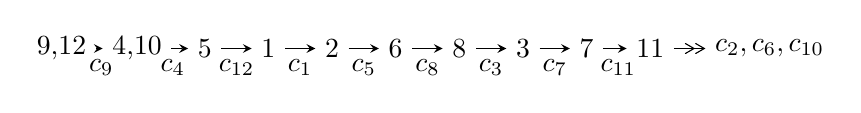
\begin{tikzpicture}[x=23pt, y=7pt]
	% node
	\node (A0) at (-1/8, 0) {9,12};
	\node (A1) at (17/16, 0) {4,10};
	\node (A2) at (17/8, 0) {5};
	\node (A3) at (25/8, 0) {1};
	\node (A4) at (33/8, 0) {2};
	\node (A5) at (41/8, 0) {6};
	\node (A6) at (49/8, 0) {8};
	\node (A7) at (57/8, 0) {3};
	\node (A8) at (65/8, 0) {7};
	\node (A9) at (73/8, 0) {11};
	\node (C1) at (1/2, -1) {$c_{9}$};
	\node (C2) at (13/8, -1) {$c_{4}$};
	\node (C3) at (21/8, -1) {$c_{12}$};
	\node (C4) at (29/8, -1) {$c_{1}$};
	\node (C5) at (37/8, -1) {$c_{5}$};
	\node (C6) at (45/8, -1) {$c_{8}$};
	\node (C7) at (53/8, -1) {$c_{3}$};
	\node (C8) at (61/8, -1) {$c_{7}$};
	\node (C9) at (69/8, -1) {$c_{11}$};
	\node (A10) at (11, 0) {$c_{2},c_{6},c_{10}$};

	% edge
	\draw[->,>=stealth]	
	(A0) edge (A1) (A1) edge (A2) (A2) edge (A3) (A3) edge (A4) (A4) edge (A5) (A5) edge (A6) (A6) edge (A7) (A7) edge (A8) (A8) edge (A9) ;
	\draw[->>,>={angle 60}]	
	(A9) edge (A10);
\end{tikzpicture} \\ 

\end{tabular} \\

\footnotetext{
The image of knot diagram is generated by the software ``\textbf{Draw programme}" developed by Andrew Bartholomew(\url{http://www.layer8.co.uk/maths/draw/index.htm\#Running-draw}), where we modified some parts for our purpose(\url{https://github.com/CATsTAILs/LinksPainter}).
}\phantom \\ \newline 
\centering \textbf{Ideals for irreducible components\footnotemark of $X_{\text{par}}$} 
 
\begin{align*}
I^u_{1}&=\langle 
5.31448\times10^{257} u^{111}-1.76917\times10^{257} u^{110}+\cdots+1.48293\times10^{257} b-1.37884\times10^{258},\\
\phantom{I^u_{1}}&\phantom{= \langle  }7.71958\times10^{259} u^{111}-1.40702\times10^{260} u^{110}+\cdots+1.48293\times10^{257} a-4.42439\times10^{260},\\
\phantom{I^u_{1}}&\phantom{= \langle  }u^{112}-2 u^{111}+\cdots-23 u+1\rangle \\
I^u_{2}&=\langle 
15997 u^{25}+41142 u^{24}+\cdots+6461 b-29882,\;15550 u^{25}+46684 u^{24}+\cdots+6461 a-54931,\\
\phantom{I^u_{2}}&\phantom{= \langle  }u^{26}+3 u^{25}+\cdots-8 u-1\rangle \\
\\
\end{align*}
\raggedright * 2 irreducible components of $\dim_{\mathbb{C}}=0$, with total 138 representations.\\
\footnotetext{All coefficients of polynomials are rational numbers. But the coefficients are sometimes approximated in decimal forms when there is not enough margin.}
\newpage
\renewcommand{\arraystretch}{1}
\centering \section*{I. $I^u_{1}= \langle 5.31\times10^{257} u^{111}-1.77\times10^{257} u^{110}+\cdots+1.48\times10^{257} b-1.38\times10^{258},\;7.72\times10^{259} u^{111}-1.41\times10^{260} u^{110}+\cdots+1.48\times10^{257} a-4.42\times10^{260},\;u^{112}-2 u^{111}+\cdots-23 u+1 \rangle$}
\flushleft \textbf{(i) Arc colorings}\\
\begin{tabular}{m{7pt} m{180pt} m{7pt} m{180pt} }
\flushright $a_{9}=$&$\begin{pmatrix}1\\0\end{pmatrix}$ \\
\flushright $a_{12}=$&$\begin{pmatrix}0\\u\end{pmatrix}$ \\
\flushright $a_{4}=$&$\begin{pmatrix}-520.564 u^{111}+948.813 u^{110}+\cdots-51467.1 u+2983.55\\-3.58378 u^{111}+1.19303 u^{110}+\cdots-267.555 u+9.29811\end{pmatrix}$ \\
\flushright $a_{10}=$&$\begin{pmatrix}1\\- u^2\end{pmatrix}$ \\
\flushright $a_{5}=$&$\begin{pmatrix}-542.410 u^{111}+984.657 u^{110}+\cdots-53337.3 u+3085.16\\-2.16416 u^{111}-7.83445 u^{110}+\cdots-108.879 u+1.44931\end{pmatrix}$ \\
\flushright $a_{1}=$&$\begin{pmatrix}u\\u\end{pmatrix}$ \\
\flushright $a_{2}=$&$\begin{pmatrix}-1056.91 u^{111}+1933.81 u^{110}+\cdots-106888. u+6250.33\\-75.7120 u^{111}+135.568 u^{110}+\cdots-8302.06 u+488.749\end{pmatrix}$ \\
\flushright $a_{6}=$&$\begin{pmatrix}-1068.16 u^{111}+1953.81 u^{110}+\cdots-107946. u+6311.12\\-77.0039 u^{111}+137.226 u^{110}+\cdots-8412.35 u+495.607\end{pmatrix}$ \\
\flushright $a_{8}=$&$\begin{pmatrix}u^2+1\\u^2\end{pmatrix}$ \\
\flushright $a_{3}=$&$\begin{pmatrix}-509.806 u^{111}+926.133 u^{110}+\cdots-50189.2 u+2902.75\\-2.58895 u^{111}-5.71626 u^{110}+\cdots-190.952 u+5.54308\end{pmatrix}$ \\
\flushright $a_{7}=$&$\begin{pmatrix}-239.300 u^{111}+439.445 u^{110}+\cdots-24450.5 u+1427.38\\38.7353 u^{111}-70.8328 u^{110}+\cdots+4055.77 u-242.400\end{pmatrix}$ \\
\flushright $a_{11}=$&$\begin{pmatrix}-665.637 u^{111}+1220.07 u^{110}+\cdots-67560.3 u+3951.81\\9.83848 u^{111}-18.3554 u^{110}+\cdots+1269.98 u-78.0166\end{pmatrix}$\\&\end{tabular}
\flushleft \textbf{(ii) Obstruction class $= -1$}\\~\\
\flushleft \textbf{(iii) Cusp Shapes $= -109.837 u^{111}+198.495 u^{110}+\cdots-11119.0 u+666.424$}\\~\\
\newpage\renewcommand{\arraystretch}{1}
\flushleft \textbf{(iv) u-Polynomials at the component}\newline \\
\begin{tabular}{m{50pt}|m{274pt}}
Crossings & \hspace{64pt}u-Polynomials at each crossing \\
\hline $$\begin{aligned}c_{1}\end{aligned}$$&$\begin{aligned}
&u^{112}-4 u^{111}+\cdots-7935981 u+3893033
\end{aligned}$\\
\hline $$\begin{aligned}c_{2},c_{5}\end{aligned}$$&$\begin{aligned}
&u^{112}+u^{111}+\cdots-5 u-1
\end{aligned}$\\
\hline $$\begin{aligned}c_{3},c_{7}\end{aligned}$$&$\begin{aligned}
&u^{112}- u^{111}+\cdots-101643 u+105943
\end{aligned}$\\
\hline $$\begin{aligned}c_{4},c_{10}\end{aligned}$$&$\begin{aligned}
&u^{112}- u^{111}+\cdots+21029 u+4019
\end{aligned}$\\
\hline $$\begin{aligned}c_{6},c_{11}\end{aligned}$$&$\begin{aligned}
&u^{112}+u^{111}+\cdots-2376 u-363
\end{aligned}$\\
\hline $$\begin{aligned}c_{8},c_{9},c_{12}\end{aligned}$$&$\begin{aligned}
&u^{112}+2 u^{111}+\cdots+23 u+1
\end{aligned}$\\
\hline
\end{tabular}\\~\\
\newpage\renewcommand{\arraystretch}{1}
\flushleft \textbf{(v) Riley Polynomials at the component}\newline \\
\begin{tabular}{m{50pt}|m{274pt}}
Crossings & \hspace{64pt}Riley Polynomials at each crossing \\
\hline $$\begin{aligned}c_{1}\end{aligned}$$&$\begin{aligned}
&y^{112}-44 y^{111}+\cdots-268247760995493 y+15155705939089
\end{aligned}$\\
\hline $$\begin{aligned}c_{2},c_{5}\end{aligned}$$&$\begin{aligned}
&y^{112}-61 y^{111}+\cdots-91 y+1
\end{aligned}$\\
\hline $$\begin{aligned}c_{3},c_{7}\end{aligned}$$&$\begin{aligned}
&y^{112}-65 y^{111}+\cdots-130189064955 y+11223919249
\end{aligned}$\\
\hline $$\begin{aligned}c_{4},c_{10}\end{aligned}$$&$\begin{aligned}
&y^{112}-45 y^{111}+\cdots-949754237 y+16152361
\end{aligned}$\\
\hline $$\begin{aligned}c_{6},c_{11}\end{aligned}$$&$\begin{aligned}
&y^{112}-63 y^{111}+\cdots-4022040 y+131769
\end{aligned}$\\
\hline $$\begin{aligned}c_{8},c_{9},c_{12}\end{aligned}$$&$\begin{aligned}
&y^{112}+110 y^{111}+\cdots-77 y+1
\end{aligned}$\\
\hline
\end{tabular}\\~\\
\newpage\flushleft \textbf{(vi) Complex Volumes and Cusp Shapes}
$$\begin{array}{c|c|c}  
\text{Solutions to }I^u_{1}& \I (\text{vol} + \sqrt{-1}CS) & \text{Cusp shape}\\
 \hline 
\begin{aligned}
u &= \phantom{-}0.888878 + 0.483069 I \\
a &= \phantom{-}0.820267 - 0.852850 I \\
b &= \phantom{-}0.105956 + 0.406692 I\end{aligned}
 & -0.75358 + 13.54180 I & \phantom{-0.000000 } 0 \\ \hline\begin{aligned}
u &= \phantom{-}0.888878 - 0.483069 I \\
a &= \phantom{-}0.820267 + 0.852850 I \\
b &= \phantom{-}0.105956 - 0.406692 I\end{aligned}
 & -0.75358 - 13.54180 I & \phantom{-0.000000 } 0 \\ \hline\begin{aligned}
u &= -0.848540 + 0.407010 I \\
a &= -0.977309 - 0.231448 I \\
b &= \phantom{-}0.164712 + 0.307819 I\end{aligned}
 & -3.28167 + 2.36912 I & \phantom{-0.000000 } 0 \\ \hline\begin{aligned}
u &= -0.848540 - 0.407010 I \\
a &= -0.977309 + 0.231448 I \\
b &= \phantom{-}0.164712 - 0.307819 I\end{aligned}
 & -3.28167 - 2.36912 I & \phantom{-0.000000 } 0 \\ \hline\begin{aligned}
u &= \phantom{-}0.984950 + 0.412034 I \\
a &= -0.768371 + 0.619947 I \\
b &= \phantom{-}0.000420 - 0.259804 I\end{aligned}
 & \phantom{-}2.27707 + 6.24115 I & \phantom{-0.000000 } 0 \\ \hline\begin{aligned}
u &= \phantom{-}0.984950 - 0.412034 I \\
a &= -0.768371 - 0.619947 I \\
b &= \phantom{-}0.000420 + 0.259804 I\end{aligned}
 & \phantom{-}2.27707 - 6.24115 I & \phantom{-0.000000 } 0 \\ \hline\begin{aligned}
u &= -0.656780 + 0.638719 I \\
a &= -0.213899 - 0.194560 I \\
b &= \phantom{-}0.359123 + 0.934305 I\end{aligned}
 & -4.15110 - 7.34468 I & \phantom{-0.000000 } 0 \\ \hline\begin{aligned}
u &= -0.656780 - 0.638719 I \\
a &= -0.213899 + 0.194560 I \\
b &= \phantom{-}0.359123 - 0.934305 I\end{aligned}
 & -4.15110 + 7.34468 I & \phantom{-0.000000 } 0 \\ \hline\begin{aligned}
u &= \phantom{-}0.309096 + 0.859738 I \\
a &= -0.683678 - 0.177668 I \\
b &= \phantom{-}0.698397 - 0.169884 I\end{aligned}
 & \phantom{-}2.04420 - 4.39389 I & \phantom{-0.000000 } 0 \\ \hline\begin{aligned}
u &= \phantom{-}0.309096 - 0.859738 I \\
a &= -0.683678 + 0.177668 I \\
b &= \phantom{-}0.698397 + 0.169884 I\end{aligned}
 & \phantom{-}2.04420 + 4.39389 I & \phantom{-0.000000 } 0\\
 \hline 
 \end{array}$$\newpage$$\begin{array}{c|c|c}  
\text{Solutions to }I^u_{1}& \I (\text{vol} + \sqrt{-1}CS) & \text{Cusp shape}\\
 \hline 
\begin{aligned}
u &= \phantom{-}0.908274\phantom{ +0.000000I} \\
a &= \phantom{-}1.24784\phantom{ +0.000000I} \\
b &= -0.295395\phantom{ +0.000000I}\end{aligned}
 & -6.60691\phantom{ +0.000000I} & \phantom{-0.000000 } 0 \\ \hline\begin{aligned}
u &= -0.892339 + 0.659239 I \\
a &= \phantom{-}0.360633 + 0.565138 I \\
b &= \phantom{-}0.005139 - 0.182725 I\end{aligned}
 & \phantom{-}0.29491 - 2.84712 I & \phantom{-0.000000 } 0 \\ \hline\begin{aligned}
u &= -0.892339 - 0.659239 I \\
a &= \phantom{-}0.360633 - 0.565138 I \\
b &= \phantom{-}0.005139 + 0.182725 I\end{aligned}
 & \phantom{-}0.29491 + 2.84712 I & \phantom{-0.000000 } 0 \\ \hline\begin{aligned}
u &= \phantom{-}0.812198 + 0.764487 I \\
a &= -0.010822 + 0.256620 I \\
b &= -0.774675 + 0.603921 I\end{aligned}
 & -1.53240 - 7.81325 I & \phantom{-0.000000 } 0 \\ \hline\begin{aligned}
u &= \phantom{-}0.812198 - 0.764487 I \\
a &= -0.010822 - 0.256620 I \\
b &= -0.774675 - 0.603921 I\end{aligned}
 & -1.53240 + 7.81325 I & \phantom{-0.000000 } 0 \\ \hline\begin{aligned}
u &= -0.721219 + 0.471928 I \\
a &= -0.83967 - 1.36144 I \\
b &= -0.076016 + 0.296520 I\end{aligned}
 & -3.81198 - 6.62535 I & \phantom{-0.000000 } 0 \\ \hline\begin{aligned}
u &= -0.721219 - 0.471928 I \\
a &= -0.83967 + 1.36144 I \\
b &= -0.076016 - 0.296520 I\end{aligned}
 & -3.81198 + 6.62535 I & \phantom{-0.000000 } 0 \\ \hline\begin{aligned}
u &= -0.692596 + 0.511227 I \\
a &= \phantom{-}0.127886 + 0.177907 I \\
b &= \phantom{-}0.963684 + 0.451851 I\end{aligned}
 & -3.97617 + 1.98114 I & \phantom{-0.000000 } 0 \\ \hline\begin{aligned}
u &= -0.692596 - 0.511227 I \\
a &= \phantom{-}0.127886 - 0.177907 I \\
b &= \phantom{-}0.963684 - 0.451851 I\end{aligned}
 & -3.97617 - 1.98114 I & \phantom{-0.000000 } 0 \\ \hline\begin{aligned}
u &= -0.827898 + 0.802767 I \\
a &= -0.226581 - 0.011489 I \\
b &= -0.474973 - 0.448407 I\end{aligned}
 & -0.07268 - 3.27898 I & \phantom{-0.000000 } 0\\
 \hline 
 \end{array}$$\newpage$$\begin{array}{c|c|c}  
\text{Solutions to }I^u_{1}& \I (\text{vol} + \sqrt{-1}CS) & \text{Cusp shape}\\
 \hline 
\begin{aligned}
u &= -0.827898 - 0.802767 I \\
a &= -0.226581 + 0.011489 I \\
b &= -0.474973 + 0.448407 I\end{aligned}
 & -0.07268 + 3.27898 I & \phantom{-0.000000 } 0 \\ \hline\begin{aligned}
u &= -0.571035 + 0.609680 I \\
a &= -0.286966 + 0.923789 I \\
b &= -0.081621 - 0.325077 I\end{aligned}
 & -0.36569 - 3.63805 I & \phantom{-0.000000 } 0 \\ \hline\begin{aligned}
u &= -0.571035 - 0.609680 I \\
a &= -0.286966 - 0.923789 I \\
b &= -0.081621 + 0.325077 I\end{aligned}
 & -0.36569 + 3.63805 I & \phantom{-0.000000 } 0 \\ \hline\begin{aligned}
u &= \phantom{-}0.415284 + 1.093070 I \\
a &= \phantom{-}0.188349 + 0.475086 I \\
b &= -0.654100 + 0.506853 I\end{aligned}
 & \phantom{-}4.02686 + 1.81633 I & \phantom{-0.000000 } 0 \\ \hline\begin{aligned}
u &= \phantom{-}0.415284 - 1.093070 I \\
a &= \phantom{-}0.188349 - 0.475086 I \\
b &= -0.654100 - 0.506853 I\end{aligned}
 & \phantom{-}4.02686 - 1.81633 I & \phantom{-0.000000 } 0 \\ \hline\begin{aligned}
u &= -0.469786 + 0.633364 I \\
a &= -0.809509 + 0.707431 I \\
b &= -0.246105 - 0.235061 I\end{aligned}
 & -0.31782 - 3.60247 I & \phantom{-0.000000 } 0 \\ \hline\begin{aligned}
u &= -0.469786 - 0.633364 I \\
a &= -0.809509 - 0.707431 I \\
b &= -0.246105 + 0.235061 I\end{aligned}
 & -0.31782 + 3.60247 I & \phantom{-0.000000 } 0 \\ \hline\begin{aligned}
u &= -0.522680 + 0.554135 I \\
a &= \phantom{-}0.073104 + 0.998642 I \\
b &= \phantom{-}0.468593 - 0.304847 I\end{aligned}
 & \phantom{-}0.73324 - 3.77410 I & \phantom{-0.000000 } 0 \\ \hline\begin{aligned}
u &= -0.522680 - 0.554135 I \\
a &= \phantom{-}0.073104 - 0.998642 I \\
b &= \phantom{-}0.468593 + 0.304847 I\end{aligned}
 & \phantom{-}0.73324 + 3.77410 I & \phantom{-0.000000 } 0 \\ \hline\begin{aligned}
u &= \phantom{-}0.584674 + 0.478117 I \\
a &= \phantom{-}0.526437 - 0.727056 I \\
b &= -0.518271 + 0.594563 I\end{aligned}
 & -7.45052 + 1.97887 I & \phantom{-0.000000 } 0\\
 \hline 
 \end{array}$$\newpage$$\begin{array}{c|c|c}  
\text{Solutions to }I^u_{1}& \I (\text{vol} + \sqrt{-1}CS) & \text{Cusp shape}\\
 \hline 
\begin{aligned}
u &= \phantom{-}0.584674 - 0.478117 I \\
a &= \phantom{-}0.526437 + 0.727056 I \\
b &= -0.518271 - 0.594563 I\end{aligned}
 & -7.45052 - 1.97887 I & \phantom{-0.000000 } 0 \\ \hline\begin{aligned}
u &= \phantom{-}0.239762 + 1.222110 I \\
a &= \phantom{-}0.903455 - 0.644187 I \\
b &= \phantom{-}2.08979 - 1.24020 I\end{aligned}
 & -1.78376 + 4.58038 I & \phantom{-0.000000 } 0 \\ \hline\begin{aligned}
u &= \phantom{-}0.239762 - 1.222110 I \\
a &= \phantom{-}0.903455 + 0.644187 I \\
b &= \phantom{-}2.08979 + 1.24020 I\end{aligned}
 & -1.78376 - 4.58038 I & \phantom{-0.000000 } 0 \\ \hline\begin{aligned}
u &= \phantom{-}0.719928 + 0.204245 I \\
a &= \phantom{-}1.073130 - 0.817359 I \\
b &= \phantom{-}0.544051 + 0.338917 I\end{aligned}
 & \phantom{-}6.62237 + 2.30625 I & \phantom{-0.000000 } 0 \\ \hline\begin{aligned}
u &= \phantom{-}0.719928 - 0.204245 I \\
a &= \phantom{-}1.073130 + 0.817359 I \\
b &= \phantom{-}0.544051 - 0.338917 I\end{aligned}
 & \phantom{-}6.62237 - 2.30625 I & \phantom{-0.000000 } 0 \\ \hline\begin{aligned}
u &= \phantom{-}0.734331 + 1.018270 I \\
a &= \phantom{-}0.220294 - 0.220908 I \\
b &= \phantom{-}0.683557 - 0.753562 I\end{aligned}
 & \phantom{-}0.526244 - 0.211571 I & \phantom{-0.000000 } 0 \\ \hline\begin{aligned}
u &= \phantom{-}0.734331 - 1.018270 I \\
a &= \phantom{-}0.220294 + 0.220908 I \\
b &= \phantom{-}0.683557 + 0.753562 I\end{aligned}
 & \phantom{-}0.526244 + 0.211571 I & \phantom{-0.000000 } 0 \\ \hline\begin{aligned}
u &= \phantom{-}0.229525 + 1.250300 I \\
a &= -0.71424 + 1.43502 I \\
b &= -1.68809 + 2.63776 I\end{aligned}
 & \phantom{-}0.56515 + 3.26255 I & \phantom{-0.000000 } 0 \\ \hline\begin{aligned}
u &= \phantom{-}0.229525 - 1.250300 I \\
a &= -0.71424 - 1.43502 I \\
b &= -1.68809 - 2.63776 I\end{aligned}
 & \phantom{-}0.56515 - 3.26255 I & \phantom{-0.000000 } 0 \\ \hline\begin{aligned}
u &= \phantom{-}0.640231 + 0.286062 I \\
a &= -0.870616 + 1.039980 I \\
b &= -0.642136 - 0.634118 I\end{aligned}
 & \phantom{-}3.72195 + 7.95714 I & \phantom{-0.000000 } 0\\
 \hline 
 \end{array}$$\newpage$$\begin{array}{c|c|c}  
\text{Solutions to }I^u_{1}& \I (\text{vol} + \sqrt{-1}CS) & \text{Cusp shape}\\
 \hline 
\begin{aligned}
u &= \phantom{-}0.640231 - 0.286062 I \\
a &= -0.870616 - 1.039980 I \\
b &= -0.642136 + 0.634118 I\end{aligned}
 & \phantom{-}3.72195 - 7.95714 I & \phantom{-0.000000 } 0 \\ \hline\begin{aligned}
u &= \phantom{-}0.065592 + 1.324340 I \\
a &= \phantom{-}1.38872 + 1.34246 I \\
b &= \phantom{-}1.94468 + 2.24119 I\end{aligned}
 & -2.68484 - 4.51466 I & \phantom{-0.000000 } 0 \\ \hline\begin{aligned}
u &= \phantom{-}0.065592 - 1.324340 I \\
a &= \phantom{-}1.38872 - 1.34246 I \\
b &= \phantom{-}1.94468 - 2.24119 I\end{aligned}
 & -2.68484 + 4.51466 I & \phantom{-0.000000 } 0 \\ \hline\begin{aligned}
u &= -0.569998 + 0.354459 I \\
a &= \phantom{-}0.068889 - 0.831964 I \\
b &= -0.564605 + 0.099910 I\end{aligned}
 & \phantom{-}1.270540 + 0.011557 I & \phantom{-0.000000 } 0 \\ \hline\begin{aligned}
u &= -0.569998 - 0.354459 I \\
a &= \phantom{-}0.068889 + 0.831964 I \\
b &= -0.564605 - 0.099910 I\end{aligned}
 & \phantom{-}1.270540 - 0.011557 I & \phantom{-0.000000 } 0 \\ \hline\begin{aligned}
u &= \phantom{-}0.667378\phantom{ +0.000000I} \\
a &= \phantom{-}2.88391\phantom{ +0.000000I} \\
b &= \phantom{-}0.210916\phantom{ +0.000000I}\end{aligned}
 & \phantom{-}4.38393\phantom{ +0.000000I} & \phantom{-0.000000 } 0 \\ \hline\begin{aligned}
u &= \phantom{-}0.187133 + 1.339810 I \\
a &= \phantom{-}0.02910 - 1.82847 I \\
b &= -0.07474 - 3.15921 I\end{aligned}
 & -2.58031 + 1.43395 I & \phantom{-0.000000 } 0 \\ \hline\begin{aligned}
u &= \phantom{-}0.187133 - 1.339810 I \\
a &= \phantom{-}0.02910 + 1.82847 I \\
b &= -0.07474 + 3.15921 I\end{aligned}
 & -2.58031 - 1.43395 I & \phantom{-0.000000 } 0 \\ \hline\begin{aligned}
u &= \phantom{-}0.038211 + 1.362560 I \\
a &= -1.03902 - 1.59308 I \\
b &= -0.91425 - 2.61426 I\end{aligned}
 & -0.909859 - 0.175020 I & \phantom{-0.000000 } 0 \\ \hline\begin{aligned}
u &= \phantom{-}0.038211 - 1.362560 I \\
a &= -1.03902 + 1.59308 I \\
b &= -0.91425 + 2.61426 I\end{aligned}
 & -0.909859 + 0.175020 I & \phantom{-0.000000 } 0\\
 \hline 
 \end{array}$$\newpage$$\begin{array}{c|c|c}  
\text{Solutions to }I^u_{1}& \I (\text{vol} + \sqrt{-1}CS) & \text{Cusp shape}\\
 \hline 
\begin{aligned}
u &= \phantom{-}0.621091 + 0.052178 I \\
a &= -2.07214 + 1.27013 I \\
b &= -0.110111 - 0.184233 I\end{aligned}
 & \phantom{-}1.78705 - 1.40064 I & \phantom{-0.000000 } 0 \\ \hline\begin{aligned}
u &= \phantom{-}0.621091 - 0.052178 I \\
a &= -2.07214 - 1.27013 I \\
b &= -0.110111 + 0.184233 I\end{aligned}
 & \phantom{-}1.78705 + 1.40064 I & \phantom{-0.000000 } 0 \\ \hline\begin{aligned}
u &= \phantom{-}0.046611 + 1.388430 I \\
a &= -0.764451 + 0.232753 I \\
b &= -2.78588 + 0.38709 I\end{aligned}
 & -2.91103 + 6.41883 I & \phantom{-0.000000 } 0 \\ \hline\begin{aligned}
u &= \phantom{-}0.046611 - 1.388430 I \\
a &= -0.764451 - 0.232753 I \\
b &= -2.78588 - 0.38709 I\end{aligned}
 & -2.91103 - 6.41883 I & \phantom{-0.000000 } 0 \\ \hline\begin{aligned}
u &= \phantom{-}0.041592 + 1.388610 I \\
a &= -0.049359 - 0.808927 I \\
b &= \phantom{-}1.31465 - 1.45004 I\end{aligned}
 & -1.11162 + 1.61071 I & \phantom{-0.000000 } 0 \\ \hline\begin{aligned}
u &= \phantom{-}0.041592 - 1.388610 I \\
a &= -0.049359 + 0.808927 I \\
b &= \phantom{-}1.31465 + 1.45004 I\end{aligned}
 & -1.11162 - 1.61071 I & \phantom{-0.000000 } 0 \\ \hline\begin{aligned}
u &= -0.216039 + 1.373150 I \\
a &= -0.597574 + 0.473238 I \\
b &= -0.891372 + 0.629845 I\end{aligned}
 & -4.09294 - 2.79139 I & \phantom{-0.000000 } 0 \\ \hline\begin{aligned}
u &= -0.216039 - 1.373150 I \\
a &= -0.597574 - 0.473238 I \\
b &= -0.891372 - 0.629845 I\end{aligned}
 & -4.09294 + 2.79139 I & \phantom{-0.000000 } 0 \\ \hline\begin{aligned}
u &= \phantom{-}0.241355 + 1.389350 I \\
a &= \phantom{-}0.36435 + 1.63142 I \\
b &= \phantom{-}0.49327 + 2.39937 I\end{aligned}
 & \phantom{-}1.53420 + 5.71848 I & \phantom{-0.000000 } 0 \\ \hline\begin{aligned}
u &= \phantom{-}0.241355 - 1.389350 I \\
a &= \phantom{-}0.36435 - 1.63142 I \\
b &= \phantom{-}0.49327 - 2.39937 I\end{aligned}
 & \phantom{-}1.53420 - 5.71848 I & \phantom{-0.000000 } 0\\
 \hline 
 \end{array}$$\newpage$$\begin{array}{c|c|c}  
\text{Solutions to }I^u_{1}& \I (\text{vol} + \sqrt{-1}CS) & \text{Cusp shape}\\
 \hline 
\begin{aligned}
u &= -0.108951 + 1.406800 I \\
a &= -0.333720 + 1.288790 I \\
b &= -0.40544 + 1.85399 I\end{aligned}
 & -4.05644 - 2.25978 I & \phantom{-0.000000 } 0 \\ \hline\begin{aligned}
u &= -0.108951 - 1.406800 I \\
a &= -0.333720 - 1.288790 I \\
b &= -0.40544 - 1.85399 I\end{aligned}
 & -4.05644 + 2.25978 I & \phantom{-0.000000 } 0 \\ \hline\begin{aligned}
u &= \phantom{-}0.034930 + 1.413010 I \\
a &= \phantom{-}1.62996 - 1.06504 I \\
b &= \phantom{-}1.06109 - 1.25473 I\end{aligned}
 & -5.63807 - 0.19831 I & \phantom{-0.000000 } 0 \\ \hline\begin{aligned}
u &= \phantom{-}0.034930 - 1.413010 I \\
a &= \phantom{-}1.62996 + 1.06504 I \\
b &= \phantom{-}1.06109 + 1.25473 I\end{aligned}
 & -5.63807 + 0.19831 I & \phantom{-0.000000 } 0 \\ \hline\begin{aligned}
u &= -0.556673 + 0.170203 I \\
a &= -0.038788 - 0.318279 I \\
b &= -0.424577 + 0.144248 I\end{aligned}
 & \phantom{-}1.029400 - 0.157780 I & \phantom{-}9.96548 + 0. I\phantom{ +0.000000I} \\ \hline\begin{aligned}
u &= -0.556673 - 0.170203 I \\
a &= -0.038788 + 0.318279 I \\
b &= -0.424577 - 0.144248 I\end{aligned}
 & \phantom{-}1.029400 + 0.157780 I & \phantom{-}9.96548 + 0. I\phantom{ +0.000000I} \\ \hline\begin{aligned}
u &= -0.01611 + 1.42034 I \\
a &= -1.27207 + 4.12698 I \\
b &= -1.23266 + 4.32374 I\end{aligned}
 & -4.86355 + 0.25606 I & \phantom{-0.000000 } 0 \\ \hline\begin{aligned}
u &= -0.01611 - 1.42034 I \\
a &= -1.27207 - 4.12698 I \\
b &= -1.23266 - 4.32374 I\end{aligned}
 & -4.86355 - 0.25606 I & \phantom{-0.000000 } 0 \\ \hline\begin{aligned}
u &= \phantom{-}0.21434 + 1.42402 I \\
a &= -0.54873 - 1.93154 I \\
b &= -0.90888 - 2.65849 I\end{aligned}
 & -1.78470 + 11.01610 I & \phantom{-0.000000 } 0 \\ \hline\begin{aligned}
u &= \phantom{-}0.21434 - 1.42402 I \\
a &= -0.54873 + 1.93154 I \\
b &= -0.90888 + 2.65849 I\end{aligned}
 & -1.78470 - 11.01610 I & \phantom{-0.000000 } 0\\
 \hline 
 \end{array}$$\newpage$$\begin{array}{c|c|c}  
\text{Solutions to }I^u_{1}& \I (\text{vol} + \sqrt{-1}CS) & \text{Cusp shape}\\
 \hline 
\begin{aligned}
u &= -0.03911 + 1.44804 I \\
a &= \phantom{-}0.18081 - 1.61496 I \\
b &= -0.20881 - 2.50376 I\end{aligned}
 & -7.08685 + 0.13972 I & \phantom{-0.000000 } 0 \\ \hline\begin{aligned}
u &= -0.03911 - 1.44804 I \\
a &= \phantom{-}0.18081 + 1.61496 I \\
b &= -0.20881 + 2.50376 I\end{aligned}
 & -7.08685 - 0.13972 I & \phantom{-0.000000 } 0 \\ \hline\begin{aligned}
u &= \phantom{-}0.40142 + 1.40893 I \\
a &= -0.441279 + 1.042440 I \\
b &= -0.46892 + 2.11084 I\end{aligned}
 & -11.17970 + 4.75221 I & \phantom{-0.000000 } 0 \\ \hline\begin{aligned}
u &= \phantom{-}0.40142 - 1.40893 I \\
a &= -0.441279 - 1.042440 I \\
b &= -0.46892 - 2.11084 I\end{aligned}
 & -11.17970 - 4.75221 I & \phantom{-0.000000 } 0 \\ \hline\begin{aligned}
u &= -0.12792 + 1.48402 I \\
a &= \phantom{-}0.77290 - 1.49329 I \\
b &= \phantom{-}1.18588 - 2.33514 I\end{aligned}
 & -5.94706 - 5.93213 I & \phantom{-0.000000 } 0 \\ \hline\begin{aligned}
u &= -0.12792 - 1.48402 I \\
a &= \phantom{-}0.77290 + 1.49329 I \\
b &= \phantom{-}1.18588 + 2.33514 I\end{aligned}
 & -5.94706 + 5.93213 I & \phantom{-0.000000 } 0 \\ \hline\begin{aligned}
u &= \phantom{-}0.18456 + 1.49371 I \\
a &= -0.51205 + 1.47476 I \\
b &= -0.14404 + 2.54769 I\end{aligned}
 & -13.8995 + 4.7412 I & \phantom{-0.000000 } 0 \\ \hline\begin{aligned}
u &= \phantom{-}0.18456 - 1.49371 I \\
a &= -0.51205 - 1.47476 I \\
b &= -0.14404 - 2.54769 I\end{aligned}
 & -13.8995 - 4.7412 I & \phantom{-0.000000 } 0 \\ \hline\begin{aligned}
u &= -0.26311 + 1.50158 I \\
a &= -0.23567 + 1.80532 I \\
b &= -0.61845 + 3.22042 I\end{aligned}
 & -10.2116 - 10.2371 I & \phantom{-0.000000 } 0 \\ \hline\begin{aligned}
u &= -0.26311 - 1.50158 I \\
a &= -0.23567 - 1.80532 I \\
b &= -0.61845 - 3.22042 I\end{aligned}
 & -10.2116 + 10.2371 I & \phantom{-0.000000 } 0\\
 \hline 
 \end{array}$$\newpage$$\begin{array}{c|c|c}  
\text{Solutions to }I^u_{1}& \I (\text{vol} + \sqrt{-1}CS) & \text{Cusp shape}\\
 \hline 
\begin{aligned}
u &= \phantom{-}0.10480 + 1.53037 I \\
a &= \phantom{-}0.266993 - 1.138530 I \\
b &= -0.27946 - 1.92995 I\end{aligned}
 & -8.14520 + 1.33211 I & \phantom{-0.000000 } 0 \\ \hline\begin{aligned}
u &= \phantom{-}0.10480 - 1.53037 I \\
a &= \phantom{-}0.266993 + 1.138530 I \\
b &= -0.27946 + 1.92995 I\end{aligned}
 & -8.14520 - 1.33211 I & \phantom{-0.000000 } 0 \\ \hline\begin{aligned}
u &= -0.065095 + 0.460437 I \\
a &= \phantom{-}1.58814 + 1.28274 I \\
b &= \phantom{-}0.479028 - 0.182021 I\end{aligned}
 & -1.165640 + 0.499413 I & -5.19076 + 1.66062 I \\ \hline\begin{aligned}
u &= -0.065095 - 0.460437 I \\
a &= \phantom{-}1.58814 - 1.28274 I \\
b &= \phantom{-}0.479028 + 0.182021 I\end{aligned}
 & -1.165640 - 0.499413 I & -5.19076 - 1.66062 I \\ \hline\begin{aligned}
u &= -0.23916 + 1.53025 I \\
a &= \phantom{-}0.659000 + 0.430745 I \\
b &= \phantom{-}0.286824 + 0.951997 I\end{aligned}
 & -10.65820 - 1.50319 I & \phantom{-0.000000 } 0 \\ \hline\begin{aligned}
u &= -0.23916 - 1.53025 I \\
a &= \phantom{-}0.659000 - 0.430745 I \\
b &= \phantom{-}0.286824 - 0.951997 I\end{aligned}
 & -10.65820 + 1.50319 I & \phantom{-0.000000 } 0 \\ \hline\begin{aligned}
u &= -0.22584 + 1.53488 I \\
a &= \phantom{-}0.350088 - 1.331390 I \\
b &= \phantom{-}0.99650 - 2.34919 I\end{aligned}
 & -7.35856 - 6.71737 I & \phantom{-0.000000 } 0 \\ \hline\begin{aligned}
u &= -0.22584 - 1.53488 I \\
a &= \phantom{-}0.350088 + 1.331390 I \\
b &= \phantom{-}0.99650 + 2.34919 I\end{aligned}
 & -7.35856 + 6.71737 I & \phantom{-0.000000 } 0 \\ \hline\begin{aligned}
u &= -0.20916 + 1.54648 I \\
a &= \phantom{-}0.51492 + 1.48797 I \\
b &= \phantom{-}0.10664 + 2.34240 I\end{aligned}
 & -11.3166 - 10.5015 I & \phantom{-0.000000 } 0 \\ \hline\begin{aligned}
u &= -0.20916 - 1.54648 I \\
a &= \phantom{-}0.51492 - 1.48797 I \\
b &= \phantom{-}0.10664 - 2.34240 I\end{aligned}
 & -11.3166 + 10.5015 I & \phantom{-0.000000 } 0\\
 \hline 
 \end{array}$$\newpage$$\begin{array}{c|c|c}  
\text{Solutions to }I^u_{1}& \I (\text{vol} + \sqrt{-1}CS) & \text{Cusp shape}\\
 \hline 
\begin{aligned}
u &= -0.21303 + 1.54923 I \\
a &= -0.048088 - 0.987232 I \\
b &= \phantom{-}0.54693 - 1.72484 I\end{aligned}
 & -7.68044 - 6.50345 I & \phantom{-0.000000 } 0 \\ \hline\begin{aligned}
u &= -0.21303 - 1.54923 I \\
a &= -0.048088 + 0.987232 I \\
b &= \phantom{-}0.54693 + 1.72484 I\end{aligned}
 & -7.68044 + 6.50345 I & \phantom{-0.000000 } 0 \\ \hline\begin{aligned}
u &= \phantom{-}0.32187 + 1.53085 I \\
a &= \phantom{-}0.15654 + 1.65884 I \\
b &= \phantom{-}0.56396 + 2.85036 I\end{aligned}
 & -7.2754 + 17.9474 I & \phantom{-0.000000 } 0 \\ \hline\begin{aligned}
u &= \phantom{-}0.32187 - 1.53085 I \\
a &= \phantom{-}0.15654 - 1.65884 I \\
b &= \phantom{-}0.56396 - 2.85036 I\end{aligned}
 & -7.2754 - 17.9474 I & \phantom{-0.000000 } 0 \\ \hline\begin{aligned}
u &= \phantom{-}0.35599 + 1.52655 I \\
a &= -0.081116 - 1.371590 I \\
b &= -0.41070 - 2.44033 I\end{aligned}
 & -4.00844 + 11.06760 I & \phantom{-0.000000 } 0 \\ \hline\begin{aligned}
u &= \phantom{-}0.35599 - 1.52655 I \\
a &= -0.081116 + 1.371590 I \\
b &= -0.41070 + 2.44033 I\end{aligned}
 & -4.00844 - 11.06760 I & \phantom{-0.000000 } 0 \\ \hline\begin{aligned}
u &= -0.32751 + 1.53359 I \\
a &= \phantom{-}0.263870 + 1.264230 I \\
b &= \phantom{-}0.24911 + 2.19387 I\end{aligned}
 & -9.58615 - 2.01979 I & \phantom{-0.000000 } 0 \\ \hline\begin{aligned}
u &= -0.32751 - 1.53359 I \\
a &= \phantom{-}0.263870 - 1.264230 I \\
b &= \phantom{-}0.24911 - 2.19387 I\end{aligned}
 & -9.58615 + 2.01979 I & \phantom{-0.000000 } 0 \\ \hline\begin{aligned}
u &= -0.24795 + 1.56918 I \\
a &= \phantom{-}0.248137 - 1.325260 I \\
b &= \phantom{-}0.69224 - 2.24165 I\end{aligned}
 & -7.09786 - 6.80459 I & \phantom{-0.000000 } 0 \\ \hline\begin{aligned}
u &= -0.24795 - 1.56918 I \\
a &= \phantom{-}0.248137 + 1.325260 I \\
b &= \phantom{-}0.69224 + 2.24165 I\end{aligned}
 & -7.09786 + 6.80459 I & \phantom{-0.000000 } 0\\
 \hline 
 \end{array}$$\newpage$$\begin{array}{c|c|c}  
\text{Solutions to }I^u_{1}& \I (\text{vol} + \sqrt{-1}CS) & \text{Cusp shape}\\
 \hline 
\begin{aligned}
u &= -0.283745 + 0.256798 I \\
a &= -0.504962 + 0.072472 I \\
b &= -0.98472 + 1.03807 I\end{aligned}
 & \phantom{-}0.425848 + 0.918121 I & \phantom{-}5.6447 + 13.0644 I \\ \hline\begin{aligned}
u &= -0.283745 - 0.256798 I \\
a &= -0.504962 - 0.072472 I \\
b &= -0.98472 - 1.03807 I\end{aligned}
 & \phantom{-}0.425848 - 0.918121 I & \phantom{-}5.6447 - 13.0644 I \\ \hline\begin{aligned}
u &= \phantom{-}0.13783 + 1.62171 I \\
a &= -0.478196 + 0.748250 I \\
b &= -0.136955 + 1.302590 I\end{aligned}
 & -9.93942 - 4.42272 I & \phantom{-0.000000 } 0 \\ \hline\begin{aligned}
u &= \phantom{-}0.13783 - 1.62171 I \\
a &= -0.478196 - 0.748250 I \\
b &= -0.136955 - 1.302590 I\end{aligned}
 & -9.93942 + 4.42272 I & \phantom{-0.000000 } 0 \\ \hline\begin{aligned}
u &= \phantom{-}0.081238 + 0.362325 I \\
a &= \phantom{-}0.93810 + 1.59958 I \\
b &= \phantom{-}0.474193 - 0.284562 I\end{aligned}
 & -1.207760 + 0.458570 I & -5.75903 - 0.46248 I \\ \hline\begin{aligned}
u &= \phantom{-}0.081238 - 0.362325 I \\
a &= \phantom{-}0.93810 - 1.59958 I \\
b &= \phantom{-}0.474193 + 0.284562 I\end{aligned}
 & -1.207760 - 0.458570 I & -5.75903 + 0.46248 I \\ \hline\begin{aligned}
u &= \phantom{-}0.117177 + 0.197063 I \\
a &= \phantom{-}1.36184 + 0.83111 I \\
b &= \phantom{-}0.98382 - 1.29410 I\end{aligned}
 & -0.385914 - 0.804745 I & -5.0743 - 22.6531 I \\ \hline\begin{aligned}
u &= \phantom{-}0.117177 - 0.197063 I \\
a &= \phantom{-}1.36184 - 0.83111 I \\
b &= \phantom{-}0.98382 + 1.29410 I\end{aligned}
 & -0.385914 + 0.804745 I & -5.0743 + 22.6531 I \\ \hline\begin{aligned}
u &= \phantom{-}0.203253 + 0.026875 I \\
a &= \phantom{-}1.99481 - 8.68595 I \\
b &= \phantom{-}0.939429 + 0.097452 I\end{aligned}
 & \phantom{-}1.73008 - 5.65394 I & \phantom{-}8.80031 + 7.77715 I \\ \hline\begin{aligned}
u &= \phantom{-}0.203253 - 0.026875 I \\
a &= \phantom{-}1.99481 + 8.68595 I \\
b &= \phantom{-}0.939429 - 0.097452 I\end{aligned}
 & \phantom{-}1.73008 + 5.65394 I & \phantom{-}8.80031 - 7.77715 I\\
 \hline 
 \end{array}$$\newpage$$\begin{array}{c|c|c}  
\text{Solutions to }I^u_{1}& \I (\text{vol} + \sqrt{-1}CS) & \text{Cusp shape}\\
 \hline 
\begin{aligned}
u &= \phantom{-}0.166581 + 0.003687 I \\
a &= -6.71770 - 5.02112 I \\
b &= -1.138890 + 0.141353 I\end{aligned}
 & \phantom{-}3.59989 + 0.92371 I & \phantom{-}5.69455 - 0.96799 I \\ \hline\begin{aligned}
u &= \phantom{-}0.166581 - 0.003687 I \\
a &= -6.71770 + 5.02112 I \\
b &= -1.138890 - 0.141353 I\end{aligned}
 & \phantom{-}3.59989 - 0.92371 I & \phantom{-}5.69455 + 0.96799 I\\
 \hline 
 \end{array}$$\newpage\newpage\renewcommand{\arraystretch}{1}
\centering \section*{II. $I^u_{2}= \langle 15997 u^{25}+41142 u^{24}+\cdots+6461 b-29882,\;15550 u^{25}+46684 u^{24}+\cdots+6461 a-54931,\;u^{26}+3 u^{25}+\cdots-8 u-1 \rangle$}
\flushleft \textbf{(i) Arc colorings}\\
\begin{tabular}{m{7pt} m{180pt} m{7pt} m{180pt} }
\flushright $a_{9}=$&$\begin{pmatrix}1\\0\end{pmatrix}$ \\
\flushright $a_{12}=$&$\begin{pmatrix}0\\u\end{pmatrix}$ \\
\flushright $a_{4}=$&$\begin{pmatrix}-2.40675 u^{25}-7.22551 u^{24}+\cdots+36.9885 u+8.50193\\-2.47593 u^{25}-6.36774 u^{24}+\cdots+19.6601 u+4.62498\end{pmatrix}$ \\
\flushright $a_{10}=$&$\begin{pmatrix}1\\- u^2\end{pmatrix}$ \\
\flushright $a_{5}=$&$\begin{pmatrix}-4.33633 u^{25}-11.6199 u^{24}+\cdots+54.1998 u+13.1217\\-2.88438 u^{25}-6.48042 u^{24}+\cdots+10.4348 u+3.23061\end{pmatrix}$ \\
\flushright $a_{1}=$&$\begin{pmatrix}u\\u\end{pmatrix}$ \\
\flushright $a_{2}=$&$\begin{pmatrix}-1.98901 u^{25}-6.63736 u^{24}+\cdots+12.8352 u+2.96703\\-1.95929 u^{25}-7.51586 u^{24}+\cdots+22.0232 u+3.79338\end{pmatrix}$ \\
\flushright $a_{6}=$&$\begin{pmatrix}-4.07398 u^{25}-12.1879 u^{24}+\cdots+36.2506 u+8.86983\\-2.52314 u^{25}-8.78471 u^{24}+\cdots+19.0020 u+3.68209\end{pmatrix}$ \\
\flushright $a_{8}=$&$\begin{pmatrix}u^2+1\\u^2\end{pmatrix}$ \\
\flushright $a_{3}=$&$\begin{pmatrix}-4.19502 u^{25}-11.9848 u^{24}+\cdots+65.9534 u+14.5146\\-2.53645 u^{25}-6.26621 u^{24}+\cdots+20.5115 u+4.94738\end{pmatrix}$ \\
\flushright $a_{7}=$&$\begin{pmatrix}-0.436155 u^{25}-1.73116 u^{24}+\cdots+1.02120 u+2.11128\\-1.06176 u^{25}-2.36186 u^{24}+\cdots+15.9686 u+4.57963\end{pmatrix}$ \\
\flushright $a_{11}=$&$\begin{pmatrix}1.76567 u^{25}+5.80235 u^{24}+\cdots-37.0766 u-4.81814\\-1.35738 u^{25}-2.49760 u^{24}+\cdots+6.19161 u+2.49466\end{pmatrix}$\\&\end{tabular}
\flushleft \textbf{(ii) Obstruction class $= 1$}\\~\\
\flushleft \textbf{(iii) Cusp Shapes $= \frac{37907}{6461} u^{25}+\frac{116252}{6461} u^{24}+\cdots+\frac{46555}{6461} u+\frac{41161}{6461}$}\\~\\
\newpage\renewcommand{\arraystretch}{1}
\flushleft \textbf{(iv) u-Polynomials at the component}\newline \\
\begin{tabular}{m{50pt}|m{274pt}}
Crossings & \hspace{64pt}u-Polynomials at each crossing \\
\hline $$\begin{aligned}c_{1}\end{aligned}$$&$\begin{aligned}
&u^{26}-9 u^{25}+\cdots+20 u-1
\end{aligned}$\\
\hline $$\begin{aligned}c_{2}\end{aligned}$$&$\begin{aligned}
&u^{26}+6 u^{25}+\cdots+6 u+1
\end{aligned}$\\
\hline $$\begin{aligned}c_{3}\end{aligned}$$&$\begin{aligned}
&u^{26}+u^{24}+\cdots-4 u+1
\end{aligned}$\\
\hline $$\begin{aligned}c_{4}\end{aligned}$$&$\begin{aligned}
&u^{26}+u^{24}+\cdots-2 u+1
\end{aligned}$\\
\hline $$\begin{aligned}c_{5}\end{aligned}$$&$\begin{aligned}
&u^{26}-6 u^{25}+\cdots-6 u+1
\end{aligned}$\\
\hline $$\begin{aligned}c_{6}\end{aligned}$$&$\begin{aligned}
&u^{26}+2 u^{25}+\cdots+u+1
\end{aligned}$\\
\hline $$\begin{aligned}c_{7}\end{aligned}$$&$\begin{aligned}
&u^{26}+u^{24}+\cdots+4 u+1
\end{aligned}$\\
\hline $$\begin{aligned}c_{8},c_{9}\end{aligned}$$&$\begin{aligned}
&u^{26}+3 u^{25}+\cdots-8 u-1
\end{aligned}$\\
\hline $$\begin{aligned}c_{10}\end{aligned}$$&$\begin{aligned}
&u^{26}+u^{24}+\cdots+2 u+1
\end{aligned}$\\
\hline $$\begin{aligned}c_{11}\end{aligned}$$&$\begin{aligned}
&u^{26}-2 u^{25}+\cdots- u+1
\end{aligned}$\\
\hline $$\begin{aligned}c_{12}\end{aligned}$$&$\begin{aligned}
&u^{26}-3 u^{25}+\cdots+8 u-1
\end{aligned}$\\
\hline
\end{tabular}\\~\\
\newpage\renewcommand{\arraystretch}{1}
\flushleft \textbf{(v) Riley Polynomials at the component}\newline \\
\begin{tabular}{m{50pt}|m{274pt}}
Crossings & \hspace{64pt}Riley Polynomials at each crossing \\
\hline $$\begin{aligned}c_{1}\end{aligned}$$&$\begin{aligned}
&y^{26}- y^{25}+\cdots-28 y+1
\end{aligned}$\\
\hline $$\begin{aligned}c_{2},c_{5}\end{aligned}$$&$\begin{aligned}
&y^{26}-14 y^{25}+\cdots-14 y+1
\end{aligned}$\\
\hline $$\begin{aligned}c_{3},c_{7}\end{aligned}$$&$\begin{aligned}
&y^{26}+2 y^{25}+\cdots-2 y+1
\end{aligned}$\\
\hline $$\begin{aligned}c_{4},c_{10}\end{aligned}$$&$\begin{aligned}
&y^{26}+2 y^{25}+\cdots-4 y+1
\end{aligned}$\\
\hline $$\begin{aligned}c_{6},c_{11}\end{aligned}$$&$\begin{aligned}
&y^{26}-20 y^{25}+\cdots-23 y+1
\end{aligned}$\\
\hline $$\begin{aligned}c_{8},c_{9},c_{12}\end{aligned}$$&$\begin{aligned}
&y^{26}+25 y^{25}+\cdots-16 y+1
\end{aligned}$\\
\hline
\end{tabular}\\~\\
\newpage\flushleft \textbf{(vi) Complex Volumes and Cusp Shapes}
$$\begin{array}{c|c|c}  
\text{Solutions to }I^u_{2}& \I (\text{vol} + \sqrt{-1}CS) & \text{Cusp shape}\\
 \hline 
\begin{aligned}
u &= \phantom{-}0.431137 + 0.906221 I \\
a &= \phantom{-}0.525034 - 0.591227 I \\
b &= \phantom{-}1.091530 - 0.895741 I\end{aligned}
 & \phantom{-}2.53235 + 2.66750 I & \phantom{-}2.71797 - 4.12988 I \\ \hline\begin{aligned}
u &= \phantom{-}0.431137 - 0.906221 I \\
a &= \phantom{-}0.525034 + 0.591227 I \\
b &= \phantom{-}1.091530 + 0.895741 I\end{aligned}
 & \phantom{-}2.53235 - 2.66750 I & \phantom{-}2.71797 + 4.12988 I \\ \hline\begin{aligned}
u &= -0.625821 + 0.774116 I \\
a &= -0.390768 + 0.069603 I \\
b &= -0.857456 - 0.155023 I\end{aligned}
 & \phantom{-}0.47651 - 1.59156 I & \phantom{-}3.09179 + 1.37031 I \\ \hline\begin{aligned}
u &= -0.625821 - 0.774116 I \\
a &= -0.390768 - 0.069603 I \\
b &= -0.857456 + 0.155023 I\end{aligned}
 & \phantom{-}0.47651 + 1.59156 I & \phantom{-}3.09179 - 1.37031 I \\ \hline\begin{aligned}
u &= \phantom{-}0.350912 + 0.982744 I \\
a &= \phantom{-}0.724535 + 0.882894 I \\
b &= \phantom{-}0.008338 + 0.328720 I\end{aligned}
 & \phantom{-}2.43763 + 0.44354 I & \phantom{-}2.62000 - 0.55350 I \\ \hline\begin{aligned}
u &= \phantom{-}0.350912 - 0.982744 I \\
a &= \phantom{-}0.724535 - 0.882894 I \\
b &= \phantom{-}0.008338 - 0.328720 I\end{aligned}
 & \phantom{-}2.43763 - 0.44354 I & \phantom{-}2.62000 + 0.55350 I \\ \hline\begin{aligned}
u &= -0.831316 + 0.756902 I \\
a &= \phantom{-}0.029481 + 0.555177 I \\
b &= -0.008560 - 0.211277 I\end{aligned}
 & \phantom{-}0.42794 - 3.89764 I & \phantom{-}7.7924 + 12.0278 I \\ \hline\begin{aligned}
u &= -0.831316 - 0.756902 I \\
a &= \phantom{-}0.029481 - 0.555177 I \\
b &= -0.008560 + 0.211277 I\end{aligned}
 & \phantom{-}0.42794 + 3.89764 I & \phantom{-}7.7924 - 12.0278 I \\ \hline\begin{aligned}
u &= -0.849486\phantom{ +0.000000I} \\
a &= -1.21471\phantom{ +0.000000I} \\
b &= \phantom{-}0.371246\phantom{ +0.000000I}\end{aligned}
 & -6.96773\phantom{ +0.000000I} & -11.6510\phantom{ +0.000000I} \\ \hline\begin{aligned}
u &= \phantom{-}0.070449 + 1.211910 I \\
a &= -1.36431 + 0.84655 I \\
b &= -3.06517 + 1.22645 I\end{aligned}
 & -1.15999 + 6.13130 I & \phantom{-}1.88516 - 7.10392 I\\
 \hline 
 \end{array}$$\newpage$$\begin{array}{c|c|c}  
\text{Solutions to }I^u_{2}& \I (\text{vol} + \sqrt{-1}CS) & \text{Cusp shape}\\
 \hline 
\begin{aligned}
u &= \phantom{-}0.070449 - 1.211910 I \\
a &= -1.36431 - 0.84655 I \\
b &= -3.06517 - 1.22645 I\end{aligned}
 & -1.15999 - 6.13130 I & \phantom{-}1.88516 + 7.10392 I \\ \hline\begin{aligned}
u &= \phantom{-}0.198476 + 1.288260 I \\
a &= \phantom{-}0.69883 - 1.53351 I \\
b &= \phantom{-}1.74962 - 2.80678 I\end{aligned}
 & \phantom{-}1.04031 + 2.89888 I & \phantom{-}6.59624 + 1.23523 I \\ \hline\begin{aligned}
u &= \phantom{-}0.198476 - 1.288260 I \\
a &= \phantom{-}0.69883 + 1.53351 I \\
b &= \phantom{-}1.74962 + 2.80678 I\end{aligned}
 & \phantom{-}1.04031 - 2.89888 I & \phantom{-}6.59624 - 1.23523 I \\ \hline\begin{aligned}
u &= -0.189235 + 1.318580 I \\
a &= -0.0005167 - 0.0414970 I \\
b &= -0.079356 - 0.419932 I\end{aligned}
 & -4.53291 - 3.09962 I & -7.39566 + 5.41041 I \\ \hline\begin{aligned}
u &= -0.189235 - 1.318580 I \\
a &= -0.0005167 + 0.0414970 I \\
b &= -0.079356 + 0.419932 I\end{aligned}
 & -4.53291 + 3.09962 I & -7.39566 - 5.41041 I \\ \hline\begin{aligned}
u &= \phantom{-}0.062411 + 0.616662 I \\
a &= -2.28838 - 0.79006 I \\
b &= \phantom{-}0.168163 - 0.402814 I\end{aligned}
 & \phantom{-}1.04818 - 5.52113 I & -2.64456 + 5.76748 I \\ \hline\begin{aligned}
u &= \phantom{-}0.062411 - 0.616662 I \\
a &= -2.28838 + 0.79006 I \\
b &= \phantom{-}0.168163 + 0.402814 I\end{aligned}
 & \phantom{-}1.04818 + 5.52113 I & -2.64456 - 5.76748 I \\ \hline\begin{aligned}
u &= \phantom{-}0.615645\phantom{ +0.000000I} \\
a &= -3.00112\phantom{ +0.000000I} \\
b &= -0.255912\phantom{ +0.000000I}\end{aligned}
 & \phantom{-}4.97554\phantom{ +0.000000I} & \phantom{-}13.3710\phantom{ +0.000000I} \\ \hline\begin{aligned}
u &= -0.022819 + 1.411910 I \\
a &= -0.31168 - 3.49706 I \\
b &= -0.29189 - 3.84914 I\end{aligned}
 & -4.95148 + 0.31707 I & -23.6637 + 3.8963 I \\ \hline\begin{aligned}
u &= -0.022819 - 1.411910 I \\
a &= -0.31168 + 3.49706 I \\
b &= -0.29189 + 3.84914 I\end{aligned}
 & -4.95148 - 0.31707 I & -23.6637 - 3.8963 I\\
 \hline 
 \end{array}$$\newpage$$\begin{array}{c|c|c}  
\text{Solutions to }I^u_{2}& \I (\text{vol} + \sqrt{-1}CS) & \text{Cusp shape}\\
 \hline 
\begin{aligned}
u &= -0.35018 + 1.43296 I \\
a &= \phantom{-}0.431703 + 1.069810 I \\
b &= \phantom{-}0.34799 + 2.11293 I\end{aligned}
 & -11.70470 - 4.38629 I & -7.27702 + 0. I\phantom{ +0.000000I} \\ \hline\begin{aligned}
u &= -0.35018 - 1.43296 I \\
a &= \phantom{-}0.431703 - 1.069810 I \\
b &= \phantom{-}0.34799 - 2.11293 I\end{aligned}
 & -11.70470 + 4.38629 I & -7.27702 + 0. I\phantom{ +0.000000I} \\ \hline\begin{aligned}
u &= -0.20834 + 1.58437 I \\
a &= \phantom{-}0.456806 - 1.211770 I \\
b &= \phantom{-}1.13875 - 2.06521 I\end{aligned}
 & -7.51272 - 7.42768 I & -5.3367 + 13.3175 I \\ \hline\begin{aligned}
u &= -0.20834 - 1.58437 I \\
a &= \phantom{-}0.456806 + 1.211770 I \\
b &= \phantom{-}1.13875 + 2.06521 I\end{aligned}
 & -7.51272 + 7.42768 I & -5.3367 - 13.3175 I \\ \hline\begin{aligned}
u &= -0.268753 + 0.037149 I \\
a &= \phantom{-}1.59717 + 0.91988 I \\
b &= -0.259630 + 0.919058 I\end{aligned}
 & -0.134077 - 1.006200 I & \phantom{-}5.75427 - 0.30798 I \\ \hline\begin{aligned}
u &= -0.268753 - 0.037149 I \\
a &= \phantom{-}1.59717 - 0.91988 I \\
b &= -0.259630 - 0.919058 I\end{aligned}
 & -0.134077 + 1.006200 I & \phantom{-}5.75427 + 0.30798 I\\
 \hline 
 \end{array}$$\newpage
\newpage\renewcommand{\arraystretch}{1}
\centering \section*{ III. u-Polynomials}
\begin{tabular}{m{50pt}|m{274pt}}
Crossings & \hspace{64pt}u-Polynomials at each crossing \\
\hline $$\begin{aligned}c_{1}\end{aligned}$$&$\begin{aligned}
&(u^{26}-9 u^{25}+\cdots+20 u-1)\\
&\cdot(u^{112}-4 u^{111}+\cdots-7935981 u+3893033)
\end{aligned}$\\
\hline $$\begin{aligned}c_{2}\end{aligned}$$&$\begin{aligned}
&(u^{26}+6 u^{25}+\cdots+6 u+1)(u^{112}+u^{111}+\cdots-5 u-1)
\end{aligned}$\\
\hline $$\begin{aligned}c_{3}\end{aligned}$$&$\begin{aligned}
&(u^{26}+u^{24}+\cdots-4 u+1)(u^{112}- u^{111}+\cdots-101643 u+105943)
\end{aligned}$\\
\hline $$\begin{aligned}c_{4}\end{aligned}$$&$\begin{aligned}
&(u^{26}+u^{24}+\cdots-2 u+1)(u^{112}- u^{111}+\cdots+21029 u+4019)
\end{aligned}$\\
\hline $$\begin{aligned}c_{5}\end{aligned}$$&$\begin{aligned}
&(u^{26}-6 u^{25}+\cdots-6 u+1)(u^{112}+u^{111}+\cdots-5 u-1)
\end{aligned}$\\
\hline $$\begin{aligned}c_{6}\end{aligned}$$&$\begin{aligned}
&(u^{26}+2 u^{25}+\cdots+u+1)(u^{112}+u^{111}+\cdots-2376 u-363)
\end{aligned}$\\
\hline $$\begin{aligned}c_{7}\end{aligned}$$&$\begin{aligned}
&(u^{26}+u^{24}+\cdots+4 u+1)(u^{112}- u^{111}+\cdots-101643 u+105943)
\end{aligned}$\\
\hline $$\begin{aligned}c_{8},c_{9}\end{aligned}$$&$\begin{aligned}
&(u^{26}+3 u^{25}+\cdots-8 u-1)(u^{112}+2 u^{111}+\cdots+23 u+1)
\end{aligned}$\\
\hline $$\begin{aligned}c_{10}\end{aligned}$$&$\begin{aligned}
&(u^{26}+u^{24}+\cdots+2 u+1)(u^{112}- u^{111}+\cdots+21029 u+4019)
\end{aligned}$\\
\hline $$\begin{aligned}c_{11}\end{aligned}$$&$\begin{aligned}
&(u^{26}-2 u^{25}+\cdots- u+1)(u^{112}+u^{111}+\cdots-2376 u-363)
\end{aligned}$\\
\hline $$\begin{aligned}c_{12}\end{aligned}$$&$\begin{aligned}
&(u^{26}-3 u^{25}+\cdots+8 u-1)(u^{112}+2 u^{111}+\cdots+23 u+1)
\end{aligned}$\\
\hline
\end{tabular}\newpage\renewcommand{\arraystretch}{1}
\centering \section*{ IV. Riley Polynomials}
\begin{tabular}{m{50pt}|m{274pt}}
Crossings & \hspace{64pt}Riley Polynomials at each crossing \\
\hline $$\begin{aligned}c_{1}\end{aligned}$$&$\begin{aligned}
&(y^{26}- y^{25}+\cdots-28 y+1)\\
&\cdot(y^{112}-44 y^{111}+\cdots-268247760995493 y+15155705939089)
\end{aligned}$\\
\hline $$\begin{aligned}c_{2},c_{5}\end{aligned}$$&$\begin{aligned}
&(y^{26}-14 y^{25}+\cdots-14 y+1)(y^{112}-61 y^{111}+\cdots-91 y+1)
\end{aligned}$\\
\hline $$\begin{aligned}c_{3},c_{7}\end{aligned}$$&$\begin{aligned}
&(y^{26}+2 y^{25}+\cdots-2 y+1)\\
&\cdot(y^{112}-65 y^{111}+\cdots-130189064955 y+11223919249)
\end{aligned}$\\
\hline $$\begin{aligned}c_{4},c_{10}\end{aligned}$$&$\begin{aligned}
&(y^{26}+2 y^{25}+\cdots-4 y+1)\\
&\cdot(y^{112}-45 y^{111}+\cdots-949754237 y+16152361)
\end{aligned}$\\
\hline $$\begin{aligned}c_{6},c_{11}\end{aligned}$$&$\begin{aligned}
&(y^{26}-20 y^{25}+\cdots-23 y+1)\\
&\cdot(y^{112}-63 y^{111}+\cdots-4022040 y+131769)
\end{aligned}$\\
\hline $$\begin{aligned}c_{8},c_{9},c_{12}\end{aligned}$$&$\begin{aligned}
&(y^{26}+25 y^{25}+\cdots-16 y+1)(y^{112}+110 y^{111}+\cdots-77 y+1)
\end{aligned}$\\
\hline
\end{tabular}
\vskip 2pc
\end{document}